\section{Functions: declaration, definition and calling}
\label{sec:func}
\begin{frame}<beamer>
    \frametitle{Outline}
    \tableofcontents[currentsection]
\end{frame}

\begin{frame}[fragile]{Overview}

\begin{columns}
\begin{column}{0.45\linewidth}
\begin{itemize}
	\item {Functions we know}
\end{itemize}
\begin{lstlisting}
int main(.);
int printf(..);
int scanf(.);
float sqrt(.);
float floor(.);
float fabs(.); 
\end{lstlisting}
\end{column}
\begin{column}{0.45\linewidth}
\begin{itemize}
	\item {Functions in math}
\end{itemize}
\begin{eqnarray}
f(x)=sin(x) \nonumber\\
g(x)=x^2 \nonumber
\end{eqnarray}
\end{column}
\end{columns}
\begin{itemize}
	\item {They are actually comparable}
	\item {Function in C is more general}
	\item {We are going to learn to organize our codes into functions (blocks)}
\end{itemize}
\end{frame}

\begin{frame}[fragile]{Advantages of function (1)}
\begin{itemize}
	\item {We are already familiar with functions}
\end{itemize}
\begin{lstlisting}
int main(.); //entrance of the program
int printf(..); //print things onto screen
int scanf(.);  //read input from keyboard
float sqrt(.); //take square root
float floor(.); //take maximum number smaller than input
float fabs(.); //take absolute value of a float number
\end{lstlisting}
\begin{itemize}
	\item {Advantages}
	\begin{itemize}
		\item {No need to repeat others work (reinvent the wheel)}
		\item {No need to write things again and again}
		\item {Your codes become cleaner}
	\end{itemize}
\end{itemize}
\end{frame}

\begin{frame}[fragile]{Introdution of function (1)}
\begin{itemize}
	\item {Let's start with a simple example}
\end{itemize}
\begin{lstlisting}
#include <stdio.h>
void hi(int i) //<---declaration of function "hi"
{
   printf("Hello %d\n", i);
}

int main()
{
   int i = 0;
   for(i = 0; i < 5; i++)
      hi(i); //<-- call function hi(int i)
   return 0; //return value to the one who calls it
}
\end{lstlisting}
\vspace{-0.15in}
\begin{itemize}
	\item {We call \textbf{hi}() inside main}
	\item {``\textbf{main}()'' cannot be called by any other function}
\end{itemize}
\end{frame}

\begin{frame}[fragile]{Declaration of function (1)}
\begin{itemize}
	\item {Declare a function for $n!$}
\end{itemize}
\begin{lstlisting}
long fact(int i); //<-- this is the declaration

int main()
{
   int i = 5, f = 0;
   f = fact(i);
   return 0; //return value to the one who calls it
}
\end{lstlisting}
\vspace{-0.15in}
\begin{itemize}
	\item {The name should be \textbf{unique}}
	\item {There is should be input parameter(s) along with the types}
	\item {There is should be output value type}
\end{itemize}
\end{frame}


\begin{frame}[fragile]{Declaration of function (2)}
\begin{itemize}
	\item {Declare a function for $n!$}
\end{itemize}
\begin{figure}
	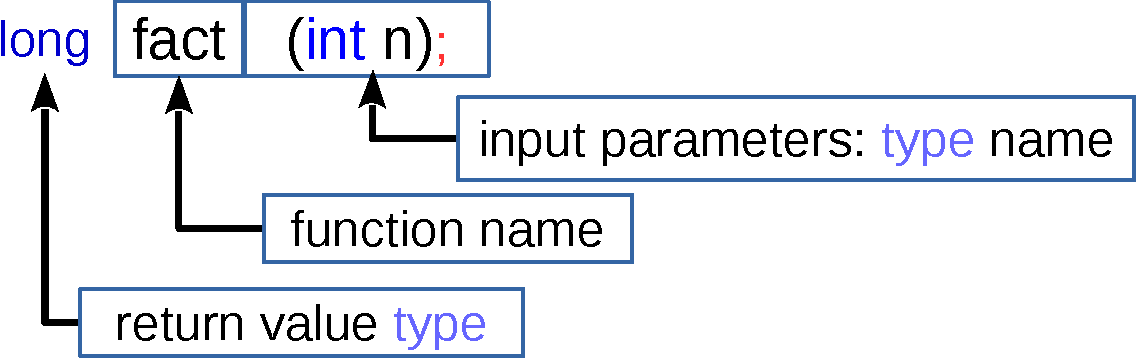
\includegraphics[width=0.8\linewidth]{figs/func_declar.pdf}
\end{figure}
\vspace{-0.15in}
\begin{itemize}
	\item {The name should be \textbf{unique}}
	\item {There should be input parameter(s) along with the types}
	\item {There should be output value type}
	\item {If there is nothing, the returning type is \textcolor{blue}{int}}
\end{itemize}
\end{frame}

\begin{frame}[fragile]{Declaration of function (3)}
\begin{itemize}
	\item {Declare a function for $n!$}
\end{itemize}
\begin{figure}
	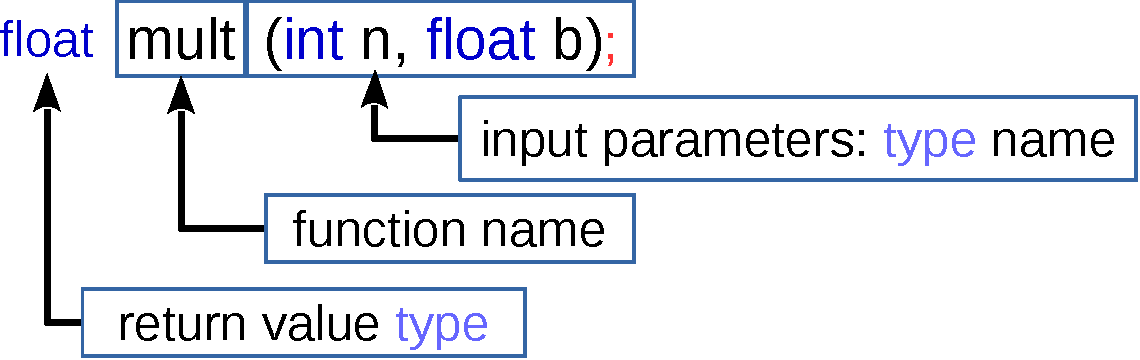
\includegraphics[width=0.8\linewidth]{figs/func_declar2.pdf}
\end{figure}
\vspace{-0.15in}
\begin{itemize}
	\item {The name should be \textbf{unique}}
	\item {There should be input parameter(s) along with the types}
	\item {There should be output value type}
	\item {If there is nothing, the returning type is \textcolor{blue}{int} by default}
\end{itemize}
\end{frame}

\begin{frame}[fragile]{Define a function (1)}
\begin{itemize}
	\item {Declare a function for $n!$}
\end{itemize}
\begin{lstlisting}
long fact(int i); //<-- this is the declaration

int main()
{
   int i = 5, f = 0;
   f = fact(i);
   return 0; //return value to the one who calls it
}
\end{lstlisting}
\vspace{-0.15in}
\begin{center}
    \Large{
	\textcolor{red}{error: undefined reference to `fact'}}
\end{center}
\begin{itemize}
	\item {``fact'' has been declared, however not defined (implemented)}
	\item {There is no function body}
	\item {When you compile it, above error comes out}
\end{itemize}

\end{frame}

\begin{frame}[fragile]{Define a function (2)}
\begin{itemize}
	\item {Declare a function for $n!$}
\end{itemize}
\begin{lstlisting}
long fact(int i); //<-- this is the declaration

int main()
{
   int i = 5;
   long f = 0;
   f = fact(i);
   return 0; //return value to the one who calls it
}
\end{lstlisting}
\vspace{-0.15in}
\begin{itemize}
	\item {Now, let's think about how to implement fact()}
\end{itemize}

\end{frame}

\begin{frame}{Define a function (3)}
	\begin{figure}
		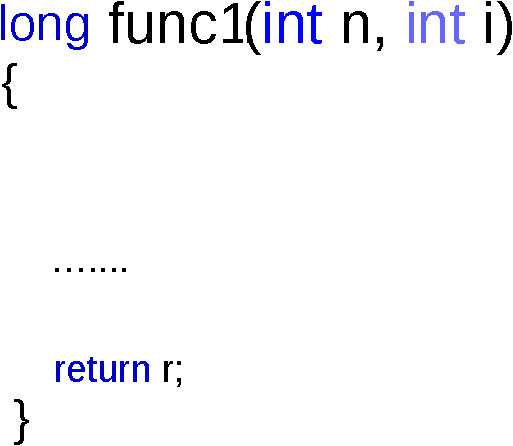
\includegraphics[width=0.35\linewidth]{figs/func_declar3.pdf}
	\end{figure}
	\begin{itemize}
		\item {You need put function implementation inside the brackets ``\{\}''}
	\end{itemize}
\end{frame}

\begin{frame}[fragile]{Define a function (4)}
\begin{itemize}
	\item {Now, let's think about how to implement fact()}
	\begin{enumerate}
		\item {For i from n to 1 do}
		\item {~~r = r*i}
		\item {~~$i--$}
		\item {End-for}
		\item {return r}
	\end{enumerate}
\end{itemize}

\end{frame}

\begin{frame}[fragile]{Define a function (4): separate declaration from definition}
\vspace{-0.2in}
\begin{columns}
\begin{column}{0.48\linewidth}
\begin{lstlisting}
long fact(int i); 
int main()
{
   int i = 5;
   long f = 0;
   f = fact(i);
   return 0; 
}
long fact(int i)
{
   long n = 1;
   if(i < 0)
     return 0;
   else if(i == 0)
     return 1;

\end{lstlisting}
\end{column}
\begin{column}{0.48\linewidth}
\begin{lstlisting}[firstnumber=16]
   else
   {
       while(i>0)
       {
          n = n*i;
          i--;
       }
   }
   return n;
}

\end{lstlisting}
\end{column}
\end{columns}
\end{frame}

\begin{frame}[fragile]{Define a function (5): combine declaration with definition}
\vspace{-0.2in}
\begin{columns}
\begin{column}{0.48\linewidth}
\begin{lstlisting}
long fact(int i)
{
   long n = 1;
   if(i < 0)
     return 0;
   else if(i == 0)
     return 1;
   else
   {
       while(i>0)
       {
          n = n*i;
          i--;
       }
   }
   return n;
}
\end{lstlisting}
\end{column}
\begin{column}{0.48\linewidth}
\begin{lstlisting}[firstnumber=18]
int main()
{
   int i = 5;
   long f = 0;
   f = fact(i);
   return 0; 
}

\end{lstlisting}
\end{column}
\end{columns}
\end{frame}

\section{Functions with Examples}
\label{sec:example}
\begin{frame}[fragile]{Example-1}
\begin{itemize}
	\item {Define a function to calculate the area of a circle}
	\item {Arguments and Parameters should be matched}
\end{itemize}
\begin{lstlisting}
float arear(float r, float pi)
{
   float a = 0;
   a = r*r*pi;
}

int main()
{
   float r = 1.5;
   const float pi = 3.1415926;
   r = area(r, pi);
   return 0;
}
\end{lstlisting}
\end{frame}

\begin{frame}[fragile]{Example-2 (1)}
\begin{itemize}
	\item {Define a function to check whether a number is Palindrome number}
	\item {such as: \textcolor{red}{321123}, \textcolor{red}{1221}, \textcolor{red}{121}}
\end{itemize}
\begin{center}
	\Large{
	Think about this in 5 minutes ...
	}
\end{center}
\end{frame}

\begin{frame}[fragile]{Example-2 (2)}
\begin{lstlisting}
int isPalindr(int n)
{
    int b = n, r = 0;
    while(b > 0){
        r = r*10+b%10;
        b = b/10;
    }
    if(n == r){
        return 1;
    }else{
        return 0;
    }
}
int main(){
   int a = 515;
   if(isPalindr(a)){
      printf("%d is Palindrome number\n", a);
   }
   return 0;
}
\end{lstlisting}
\end{frame}



\begin{frame}[fragile]{Example-3: perfect number (1)}
\begin{itemize}
	\item {1. Define a function to jugde whether an integer is a \textbf{perfect number}}
	\item {Perfect number: number equals to the sum of all its factors}
	\item {6 = 1 + 2 + 3}
	\item {2. Call it to output all the perfect numbers in range [2, 300]}
\end{itemize}
\begin{center}
	\Large{Think about this problem in 5 minutes...}
\end{center}
\end{frame}

\begin{frame}[fragile]{Example-3: perfect number (2)}
\begin{itemize}
	\item {1. Define a function to jugde whether an integer is a \textbf{perfect number}}
	\item {Perfect number: number equals to the sum of all its factors}
	\item {6 = 1 + 2 + 3}
	\item {2. Call it to output all the perfect numbers in range [2, 300]}
\end{itemize}
\begin{enumerate}
	\item {Given a number}
	\item {We should work out all its factors}
	\item {Sum all the factors up}
	\item {See whether it is equal to the number}
	\item {We should use \% operator a lot}
\end{enumerate}
\end{frame}

\begin{frame}[fragile]{Example-3: perfect number (3)}
\begin{itemize}
	\item {1. Define a function to jugde whether an integer is a \textbf{perfect number}}
	\item {\textbf{Perfect number}: number equals to the sum of all its factors}
	\item {6 = 1 + 2 + 3}
	\item {2. Call it to output all the perfect numbers in range [2, 300]}
	\item {Steps:}
	\begin{enumerate}
		\item {Give n}
		\item {~~For i from 2 to n do}
		\item {~~~~check whether n is dividable by i}
		\item {~~~~if yes, sum up}
		\item {~~Check wether sum equals to n}
		\item {~~Return \textcolor{red}{1} or \textcolor{red}{0}}
	\end{enumerate}
	\item {Let's do it now!!}
\end{itemize}
\end{frame}

\begin{frame}[fragile]{Example-3: perfect number (4)}
\vspace{-0.15in}
\begin{columns}
\begin{column}{0.55\linewidth}
\begin{enumerate}
	\item {Give n}
	\item {~~For i from 2 to n do}
	\item {~~~~check whether n is dividable by i}
	\item {~~~~if yes, sum up}
	\item {~~Check wether sum equals to n}
	\item {~~Return \textcolor{red}{1} or \textcolor{red}{0}}
\end{enumerate}
\end{column}
\begin{column}{0.45\linewidth}
\begin{lstlisting}
int isPerfect(int n)
{
    int i = 0, sum = 1;
    int up = ceil(n/2.0);
    for(i = 2; i < up; i++)
    {
        if(n%i == 0)
        {
           sum += i;
        }
    }
    if(sum == n)
      return 1;
    else 
      return 0;
}
\end{lstlisting}
\end{column}
\end{columns}
\end{frame}

\begin{frame}[fragile]{Example-3: perfect number (5)}
\vspace{-0.16in}
\begin{columns}
\begin{column}{0.48\linewidth}
\begin{lstlisting}[linewidth=0.95\linewidth]
#include <stdio.h>
#include <math.h>
int isPerfect(int n)
{
    int i = 0, sum = 1;
    int up = ceil(sqrt(n));
    for(i = 2; i < up; i++)
    {
        if(n%i == 0)
        {
           sum += i;
        }
    }
    if(sum == n)
      return 1;
    else 
      return 0;
}
\end{lstlisting}
\end{column}
\begin{column}{0.48\linewidth}
\begin{lstlisting}[firstnumber=19, linewidth=0.95\linewidth]
int main()
{
   int i = 0;
   for(i = 2; i <= 300; i++)
   {
      if(isPerfect(i))
      {
         printf("%d\n", i);
      }
   }
   return 0;
}
\end{lstlisting}
\end{column}
\end{columns}
\end{frame}



\begin{frame}[fragile]{Example-4: Armstrong number (1)}
\vspace{-0.16in}
\begin{itemize}
	\item {Define a function to check whether a number is Amstrong number}
	\item {For one digits: $1^1$ = 1}
	\item {For three digits: $1^3$ + $5^3$+$3^3$ = 153}
	\item {For four digits: $1^4 + 6^4 + 3^4 + 4^4$ = 1634}
\end{itemize}
\begin{center}
	\Large{
	   Think about this in 5 minutes ...
	}
\end{center}
\end{frame}

\begin{frame}[fragile]{Example-4: Armstrong number (2)}
\vspace{-0.16in}
\begin{columns}
\begin{column}{0.48\linewidth}
\begin{lstlisting}[linewidth=0.95\linewidth]
#include <stdio.h>
int isArms(int n)
{
  int nd = 0, s = 0, b = 0;
  int a = n, i = 0, t = 0;
  while(a > 0){
     a = a/10;
     nd++;
  }
  a = n;
  while(a > 0){
    b = a%10;
    t = 1;
    for(i = 0; i < nd; i++){
       t = t*b;
    }
    s += t;
    a  = a/10;
  }//end-while(a)
\end{lstlisting}
\end{column}
\begin{column}{0.48\linewidth}
\begin{lstlisting}[firstnumber=20, linewidth=0.95\linewidth]
   if(s == n)
     return 1;
   else
     return 0;
}

int main()
{
 int i = 1;
 for(i=1; i<100000; i++)
 {
     if(isArms(i) == 1)
     {
        printf("%6d ", i);
     }
 }
 return 0;
}
\end{lstlisting}
\end{column}
\end{columns}
\end{frame}


\begin{frame}[fragile]{Function definition: a summary}
\LARGE{
\begin{itemize}
	\item {Princeples in function definition}
	\begin{enumerate}
		\item {Remember return type, if there is no need, put \textcolor{blue}{void}}
		\item {Give a unique and self-telling name to your function}
		\item {Define function first, then you can call it (just as variable in C)}
		\item {Parameters along with the type appear in pair}
		\item {Parameters are transferred by \textcolor{red}{value}}
	\end{enumerate}
\end{itemize}
}
\end{frame}

\begin{frame}[fragile]{Parameter Transfer (1)}
\begin{figure}
	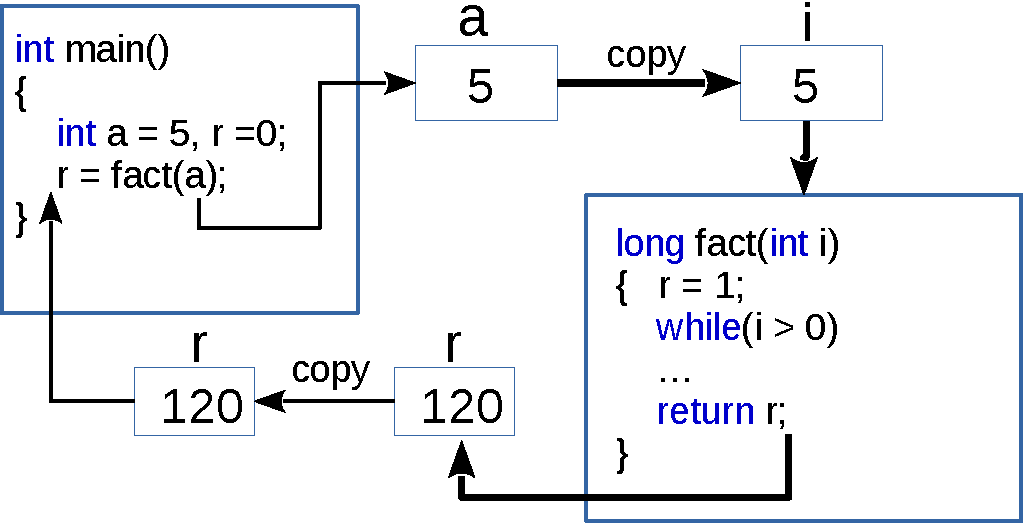
\includegraphics[width=0.85\linewidth]{figs/arg2para.pdf}
\end{figure}
\begin{itemize}
	\item {Parameters are transferred in \textcolor{red}{by value} not \textbf{by address}}
\end{itemize}
\end{frame}

\begin{frame}[fragile]{Parameter Transfer (2)}
\begin{itemize}
	\item {Let's consider a simple coding problem}
	\item {Given integers \textit{a} and \textit{b}}
	\item {You are required to swap their values}
	\item {For example, a = 5, b = 8}
	\item {After swapping, it becomes a = 8, b = 5}
\end{itemize}

\end{frame}

\begin{frame}[fragile]{Parameter Transfer (3)}
\begin{itemize}
	\item {You are required to swap their values}
	\item {For example, a = 5, b = 8}
	\item {After swapping, it becomes a = 8, b = 5}
\end{itemize}
\begin{lstlisting}
int main()
{
    int a = 5, b = 8;
    int tmp;
    printf("a = %d, b = %d\n", a, b);
    tmp = a; a = b;
    b = tmp;
    printf("a = %d, b = %d\n", a, b);
    return 0;
}
\end{lstlisting}

\end{frame}

\begin{frame}[fragile]{Parameter Transfer (4)}
\begin{itemize}
	\item {Now, let's do it by a function}
\end{itemize}
\begin{lstlisting}
#include <stdio.h>
void swap(int a, int b)
{
   int tmp = a;
   a = b; b = tmp;
   return ;
}
int main()
{
    int a = 5, b = 8;
    printf("a = %d, b = %d\n", a, b);
    swap(a, b);
    printf("a = %d, b = %d\n", a, b);
}
\end{lstlisting}
\end{frame}

\begin{frame}[fragile]{Parameter Transfer (5)}
\begin{itemize}
	\item {The result is against our will, why???}
\end{itemize}
\begin{columns}
\begin{column}{0.65\linewidth}
\begin{lstlisting}
#include <stdio.h>
void swap(int a, int b)
{
   int tmp = a;
   a = b; b = tmp;
   return ;
}
int main()
{
    int a = 5, b = 8;
    printf("a = %d, b = %d\n", a, b);
    swap(a, b);
    printf("a = %d, b = %d\n", a, b);
    return 0;
}
\end{lstlisting}
\end{column}
\begin{column}{0.3\linewidth}
[Output:]
\begin{lstlisting}
a = 5, b = 8
a = 5, b = 8
\end{lstlisting}
\end{column}
\end{columns}
\end{frame}

\begin{frame}[fragile]{Parameter Transfer (6)}
\begin{figure}
	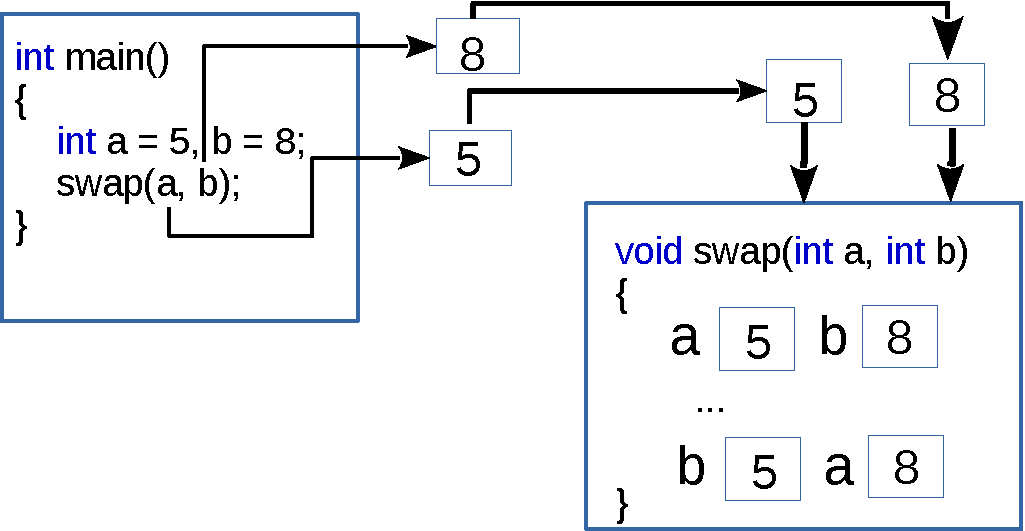
\includegraphics[width=0.85\linewidth]{figs/swap.pdf}
\end{figure}
\begin{itemize}
	\item {Parameters are transferred in \textcolor{red}{by value} not \textbf{by address}}
\end{itemize}
\end{frame}

\begin{frame}[fragile]{Function Calling again (1)}
\begin{figure}
	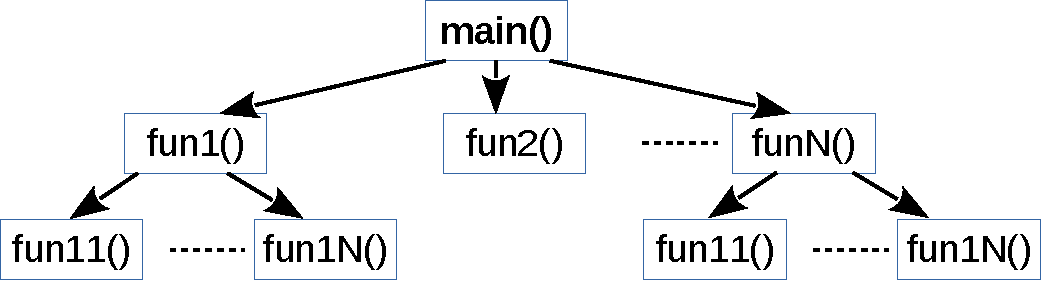
\includegraphics[width=0.8\linewidth]{figs/func_call.pdf}
\end{figure}
\begin{itemize}
	\item {Function can be called in a cascaded manner}
	\item {`main' cannot be called}
	\item {Functions are not necessarily called by `main' directly}
\end{itemize}
\end{frame}

\begin{frame}[fragile]{Function Calling again (2)}
\begin{itemize}
	\item {Parameters are transferred in \textcolor{red}{by value} not \textbf{by address}}
	\item {Arguments and Parameters should be matched}
\end{itemize}
\begin{lstlisting}
float calc(int n, float a, short int c)
{
    return (a*a*n+c);
}
int main()
{
   int n = 2;
   short int w = 4;
   float x = 4.12, r = 0;
   r = 3*calc(n, x, w);
   return 0;
}
\end{lstlisting}
\end{frame}